\documentclass{article}
\usepackage{arxiv}

\usepackage[utf8]{inputenc}
\usepackage[english, russian]{babel}
\usepackage[T1]{fontenc}
\usepackage{url}
\usepackage{booktabs}
\usepackage{amsfonts}
\usepackage{nicefrac}
\usepackage{microtype}
\usepackage{lipsum}
\usepackage{graphicx}
\usepackage{natbib}
\usepackage[unicode, colorlinks, linkcolor=Black]{hyperref}
\usepackage{doi}
\usepackage{natbib}


\title{Генерация признаков для распознавания почерка в рукописных документах}

\author{Кадченко Иван Евгеньевич \\
	ВМК МГУ\\
	\texttt{kadchenko.ivan@mail.ru} \\
	%% examples of more authors
	\And
	Местецкий Леонид Моисеевич \\
	ВМК МГУ\\
	\texttt{mestlm@mail.ru} \\
	%% \AND
	%% Coauthor \\
	%% Affiliation \\
	%% Address \\
	%% \texttt{email} \\
	%% \And
	%% Coauthor \\
	%% Affiliation \\
	%% Address \\
	%% \texttt{email} \\
	%% \And
	%% Coauthor \\
	%% Affiliation \\
	%% Address \\
	%% \texttt{email} \\
}
\date{2023}

\renewcommand{\shorttitle}{Генерация признаков для распознавания почерка в рукописных документах}

%%% Add PDF metadata to help others organize their library
%%% Once the PDF is generated, you can check the metadata with
%%% $ pdfinfo template.pdf
\hypersetup{
pdftitle={Генерация признаков для распознавания почерка в рукописных документах},
pdfsubject={q-bio.NC, q-bio.QM},
pdfauthor={Кадченко И.Е., Местецкий Л.М.},
pdfkeywords={First keyword, Second keyword, More},
}

\begin{document}
\maketitle

\begin{abstract}
	В данной работе предлагается метод распознавания почерка человека по его уникальному набору шаблонов. Пусть даны изображения рукописного текста и требуется определить, какое количество различных авторов представлено на входных изображениях и к какому автору принадлежит каждый отдельный фрагмент текста. Решение данной задачи позволит устанавливать авторства различных документов, в том числе и исторических, а также упростить работу с архивами в целом. Предлагаемое решение опирается на штриховое представление рукописного текста. Гипотеза заключается в том, что каждый человек при написании различных букв использует примерно похожие, свойственнные именно ему движения руки, а также, что у большинства людей присутствуют какие-то штрихи, выделяющие конкретного автора.
\end{abstract}


\keywords{Распознавание почерка \and Шаблоны писателя \and Рукописные документы}

\section{Введение}
Задача идентификации автора конкретного почерка ставилась с давних времён. Начиная с 5-6 веков в законодательстве Византии находило закрепление исследование почерка в судебных целях, а в России уже в XV веке при установлении подлинности документов использовалось сравнение рукописей. Ближе к настоящему времени, прикладных задач становилось всё больше. Работа с разного рода документами, от рецептов врачей до исторических скриптов, судебная аналитика и криминалистика - все эти области могут потребовать установить авторство или подлинность текста. Несмотря на всё большую цифровизацию нашей жизни, во всех упомянутых областях всё ещё используются рукописные тексты, а потому задача идентификации автора по его почерку по-прежнему сохраняется.

Распознавание почерка является одним из важнейших инструментов криминалистики, позволяющим идентифицировать автора документа или записи. Однако, существующие методы распознавания почерка требуют наличия текстовых образцов написания конкретного писателя, что затрудняет их применение в ряде случаев. В связи с этим, возникает необходимость в разработке методов распознавания почерка, которые не зависят от конкретного текста.

Один из таких методов - использование избыточных шаблонов, основанный на том, что каждый человек имеет свой индивидуальный почерк, который проявляется в определенных чертах написания букв и цифр \citep{2010PatRe..43.3853S}. Эти черты могут быть выделены из большого числа образцов почерка и использованы для создания уникального шаблона писателя.

Актуальность проблемы независимого от текста распознавания почерка заключается в том, что это может помочь ускорить и улучшить процесс идентификации автора документов и записей. Например, при расследовании преступлений, где имеется только небольшой фрагмент написанного текста, использование избыточных шаблонов может значительно сократить время на поиск подходящих образцов почерка для сравнения \citep{inbook}. Кроме того, этот метод может быть полезен при работе с историческими документами или при анализе письменных свидетельств в судебных процессах. Таким образом, разработка методов независимого от текста распознавания почерка является актуальной и важной задачей для криминалистики и других областей, где требуется идентификация авторства документов и записей.

Данная работа будет направлена на поиск признаков для создания такого уникального шаблона писателя.

\section{Постановка задачи}
Статья опирается на следующее предположение: идентификация автора по его почерку в большей степени зависит не от способа рисования или сегментации символов, когда извлеченные графемы могут нести некоторую семантическую информацию, а от физического способа создания линий или петель. Это означает, что масштаб рассматриваемых единиц письменности будет меньше. Иными словами, мы считаем, что писатель может использовать один и тот же жест рукой и, следовательно, один и тот же шаблон при написании разных символов, имеющих сходные базовые формы, как, например, одинаковые петли у разных букв (рис.1). Такие единицы письменности и назовём "штрихами".
\begin{figure}[h]
    \centering
    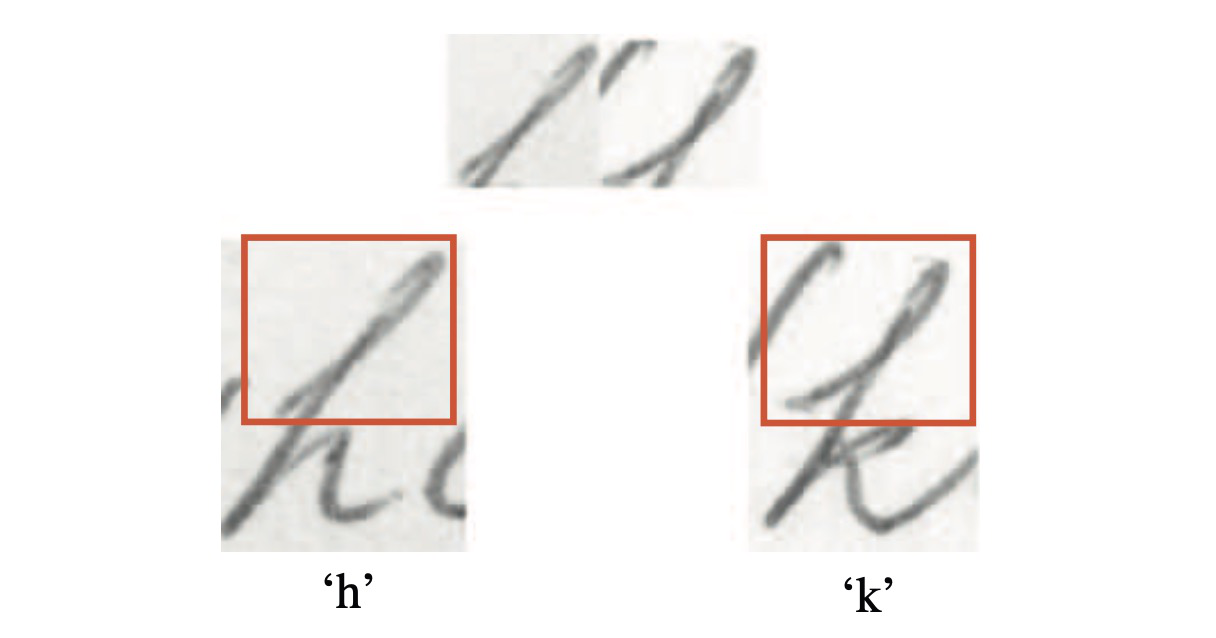
\includegraphics[width=0.8\textwidth]{rings.png}
    \caption{Одинаковые петли у двух разных букв.}
\end{figure}

Основной задачей данной работы будет являться оценка возможности классификации почерков по шаблонности и уникальности штрихов для каждого автора.

\section{Признак строк без опоры на графемы}
Как утверждалось ранее, поставлена гипотеза, что с помощью штрихового представления можно отличать почерки разных людей. Опустимся ниже в иерархии представления рукописного текста и проанализируем межстрочные и межсимвольные расстояния. 

Предлагается построить признак, отвечающий за плотность чёрных пикселей, просто просуммировав чёрные пиксели вдоль оси ординат (рис.2).

\begin{figure}[h]
\begin{minipage}[h]{0.48\linewidth}
    \centering
    \includegraphics[scale=0.25]{test2-afterotsu.jpg} 
\end{minipage}
\hfill
\begin{minipage}[h]{0.48\linewidth}
    \centering
    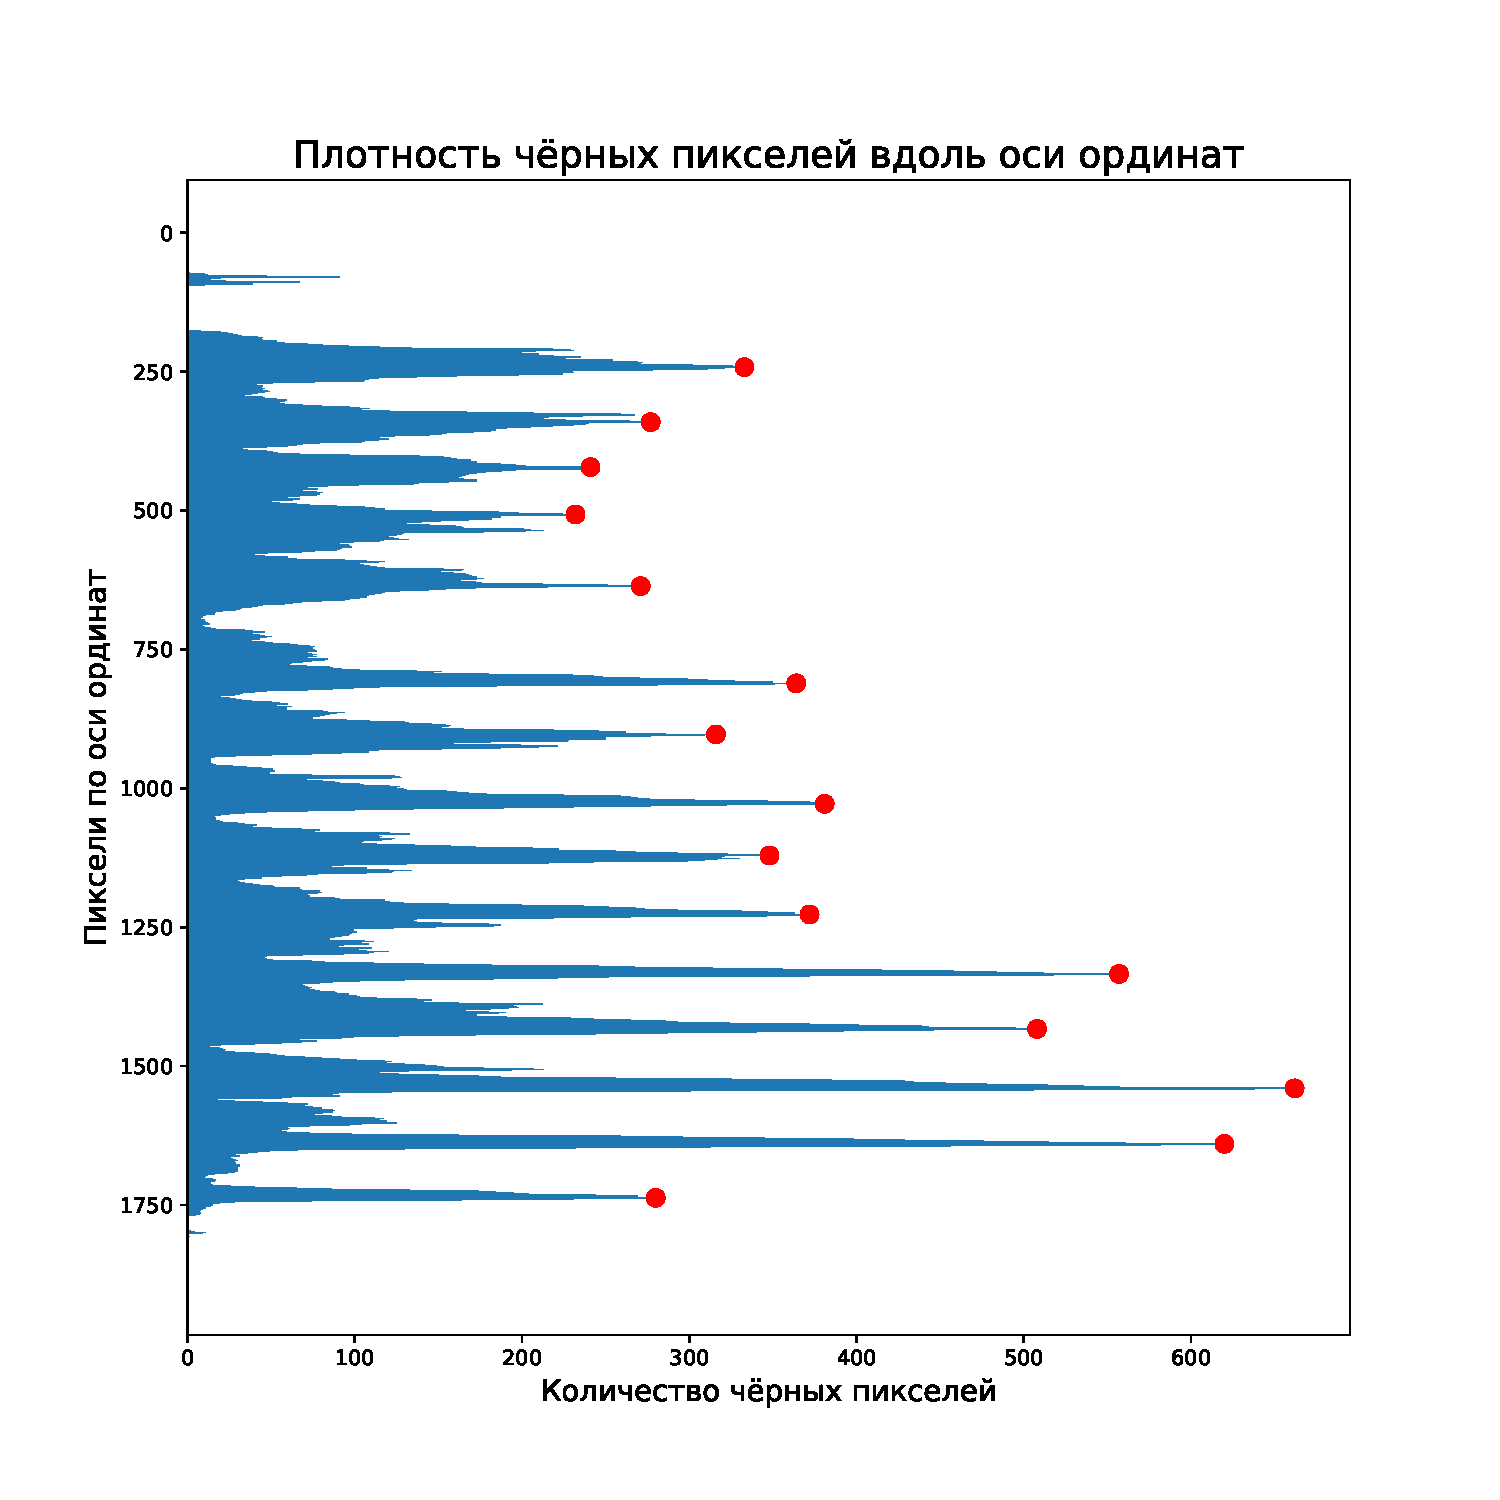
\includegraphics[scale=0.32]{density.pdf}
\end{minipage}
\caption{Рукописный текст и его плотность.}
\end{figure}

На исходном рукописном тексте можно распознать два разных почерка: первый - это первые пять строк, второй - все оставшиеся. Вытянутые столбцы на графике соответствуют строкам исходного текста, их количество совпадает. 

Построим разбиение по оси ординат по точкам глобальных минимумов на отрезках между красными точками. Также добавим в разбиение две крайние точки соответствующие примерно 150 и 1850 ординатам. Каждая из полученных областей из разбиения будет содержать ровно одну красную точку, на которой будет достигаться максимум этого отрезка.

Можно выделить два типа распределения таких областей: первые пять точек экстремума (они обозначены красными точками) с окрестностями и десять последующих. Первый тип характеризуется меньшими абсолютными значениями в точке максимума и большими абсолютными значениями в точках минимума относительно второго типа, хвосты у первого типа более тяжёлые. На основе приведённых замечаний можно однозначно установить, что на исследуемом изображении рукописного текста представлено два автора. 

Описанный подход оказывается действенным, подходящим для применения одновременно с несколькими другими признаками для создания уникального шаблона автора в поставленной ранее задаче определения количества различных почерков. Но признак имеет существенное ограничение: его разумно использовать в случае, когда строки рукописного текста близки к горизонтальному расположению, что, очевидно, выполняется далеко не всегда.

\section{Генерация признаков на основе штрихового представления}
\subsection{Сегментация по штрихам}
Для построения штрихового представления рукописного почерка на изображении будет использована программа \emph{Л.М.Местецкого}, принцип работы которой описан в источнике [3].
Пример работы программы отражён на рис.3. 

\begin{figure}[h]
\begin{minipage}[h]{1\linewidth}
\center{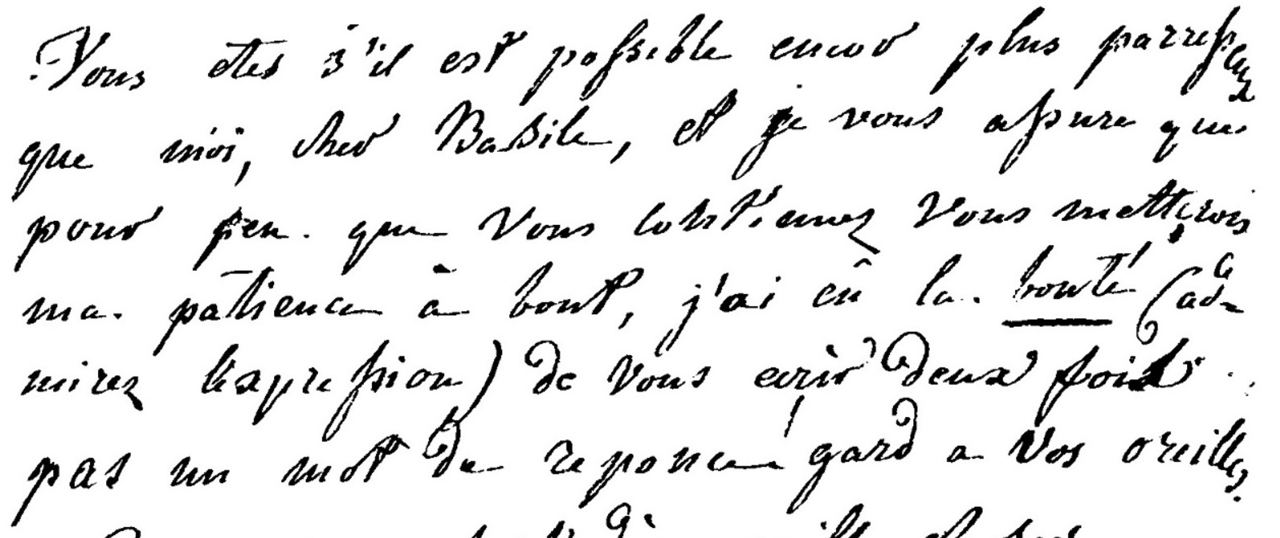
\includegraphics[width=0.95\linewidth]{4-edited.jpg}}
\end{minipage}
\vfill
\vspace{0.5cm}
\begin{minipage}[h]{1\linewidth}
\center{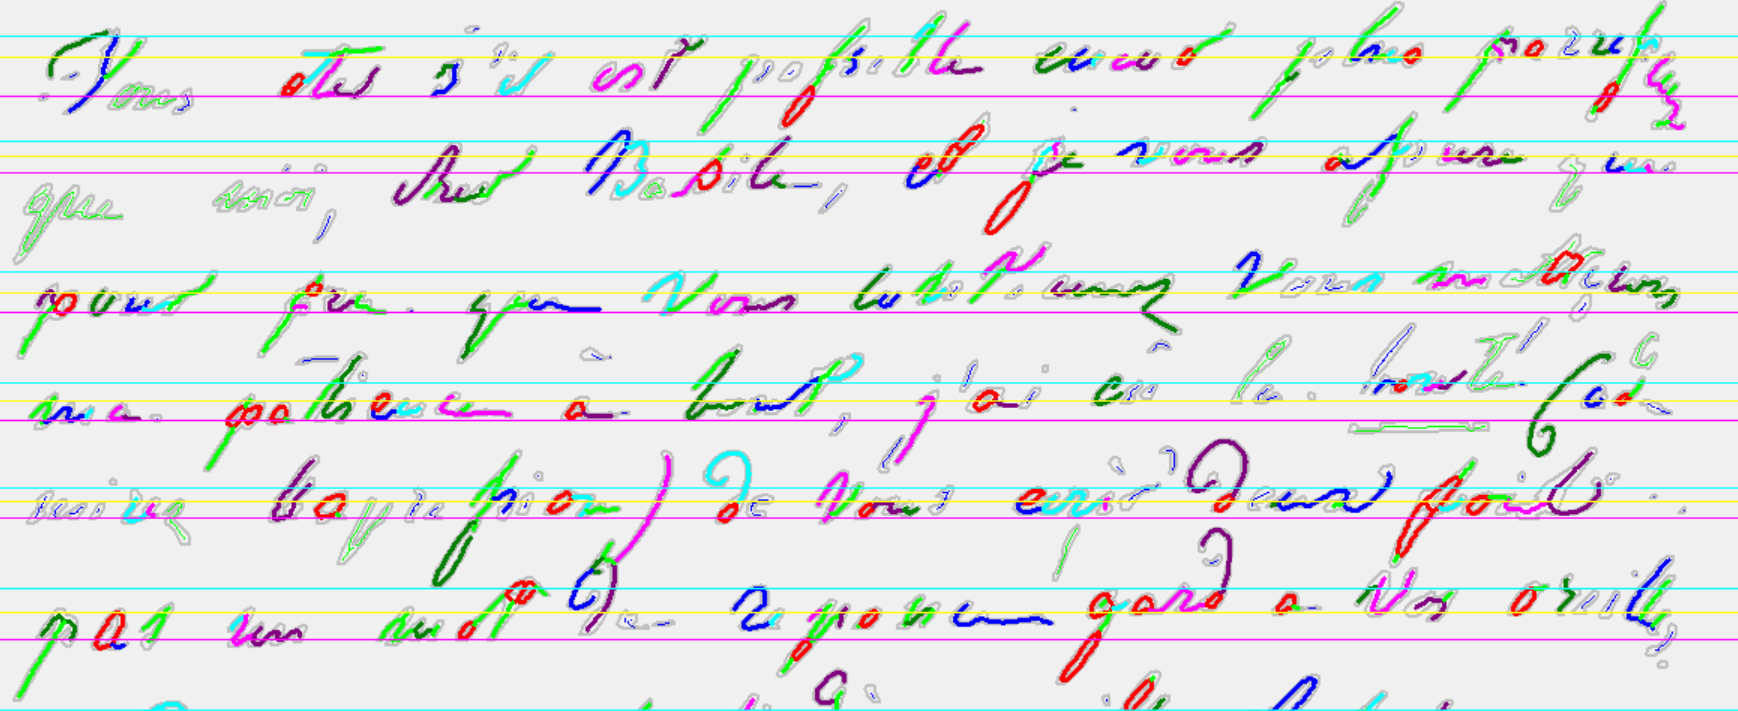
\includegraphics[width=0.95\linewidth]{example_strokes.jpg}}
\end{minipage}
\caption{Исходный рукописный текст и визуализированные штрихи.}
\end{figure}

Программа получает на вход изображение рукописного текста, бинаризует его и строит штриховое представление исходного текста, визуализируя, как на рис.3, и записывая в текстовый файл результат. Каждый штрих представляет собой набор нецелочисленных координат точек, из которых состоит штрих, и информацию о взаимном расположении этих точек, такую как тип штриха (цепь, кольцо или отрезок), его уровень (выступающий, базовый или свисающий) и номер строки, к которой штрих относится. 

Используя приведённую информацию о штрихах, постараемся построить полезные признаки, позволяющие оценить возможность классификации почерка по отдельным штрихам.

\subsection{Агрегация штрихов: наклон и кривизна}
Базовыми признаками, рассматриваемыми в задаче распознавания почерка, являются наклон и кривизна текста. Эти признаки являются стабильными параметрами [4] при допущении, что рассматриваемый документ представляет собой естественный стиль письма писателя, а не является поддельным. 

Проанализируем применимость данных характеристик при оперировании штриховым представлением. 
\subsubsection{Признак-наклон}
Имея набор пар координат точек, из которых состоит отдельный штрих, величину наклона можно определить как коэффициент \emph{incline} в модели линейной регрессии с одной независимой переменной:

\begin{equation}
y = \emph{inline}~ x + \emph{bias}
\end{equation}

Выражая из этого уравнения \emph{incline} и подставляя данные точки штрихов, можно получить формулу для вычисления наклона, смещение интересовать нас не будет:

\begin{equation}
\emph{incline} = \frac{\sum_{i=1}^{N}(x_i - \mathbb{E}x)(y_i - \mathbb{E}y)}{\sum_{i=1}^{N}(x_i - \mathbb{E}x)^2}
\end{equation}

Репрезентативность такого подхода можно наблюдать на рис.4. Распределения величины наклона для строк текста одного (1-5 строки) и другого (6-15 строки) почерка заметно отличаются. Второй почерк имеет выраженный наклон по сравнению с первым, что и отражено на графике смещением центра распределения. 

\begin{figure}[h]
\begin{minipage}[h]{0.5\linewidth}
    \centering
    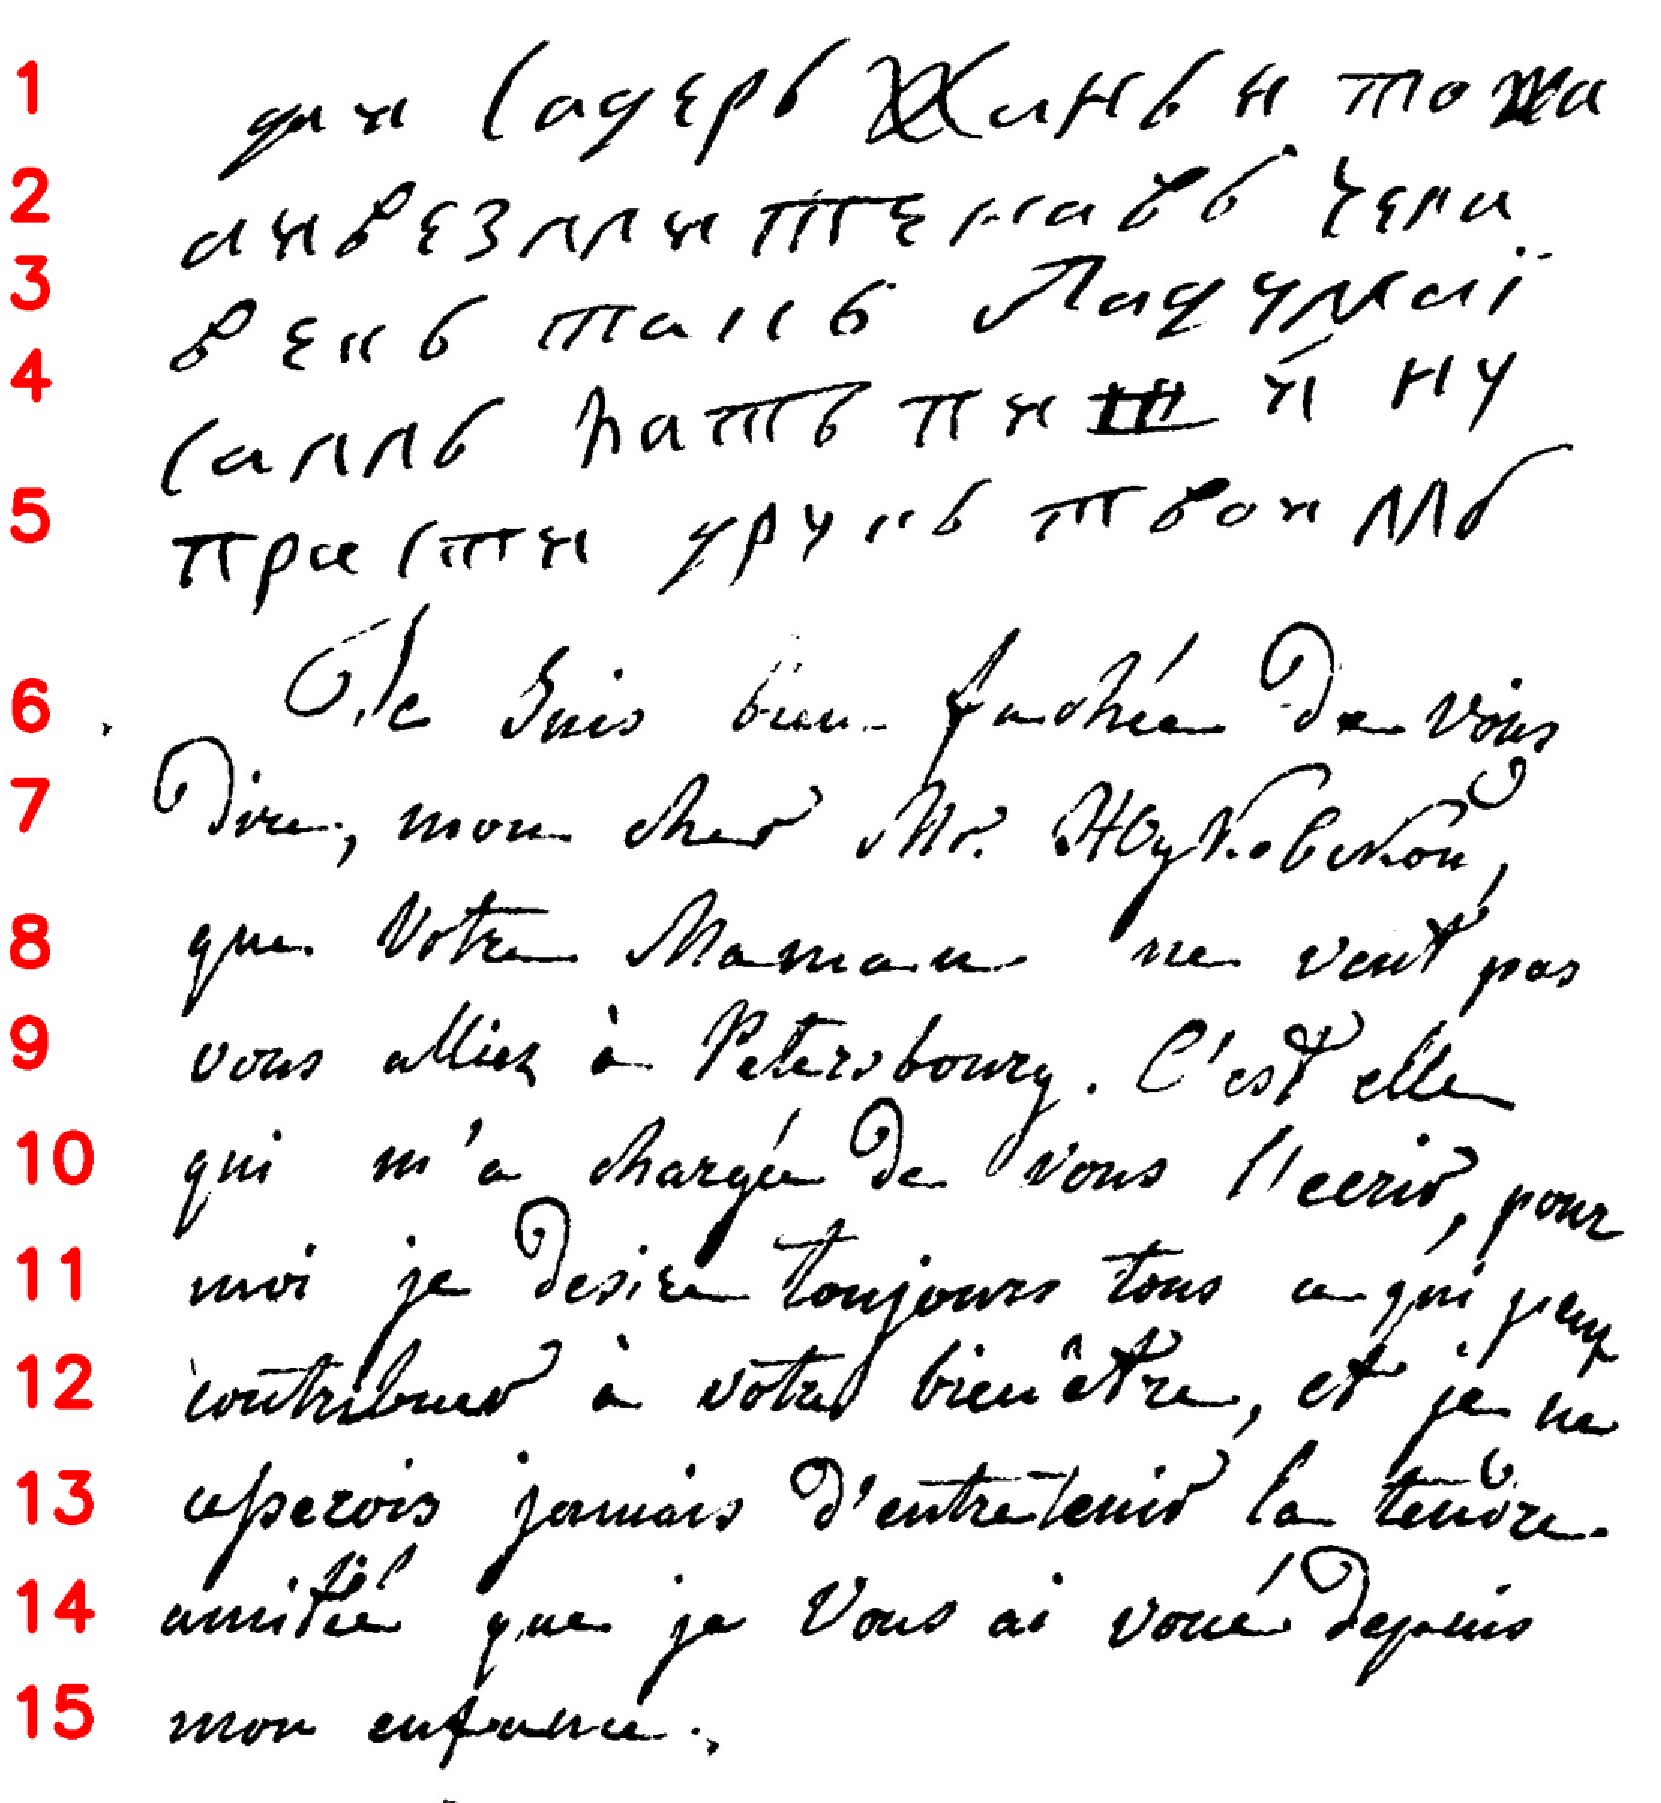
\includegraphics[scale=0.26]{afterotsu-cropped.pdf} 
\end{minipage}
\hfill
\begin{minipage}[h]{0.46\linewidth}
    \centering
    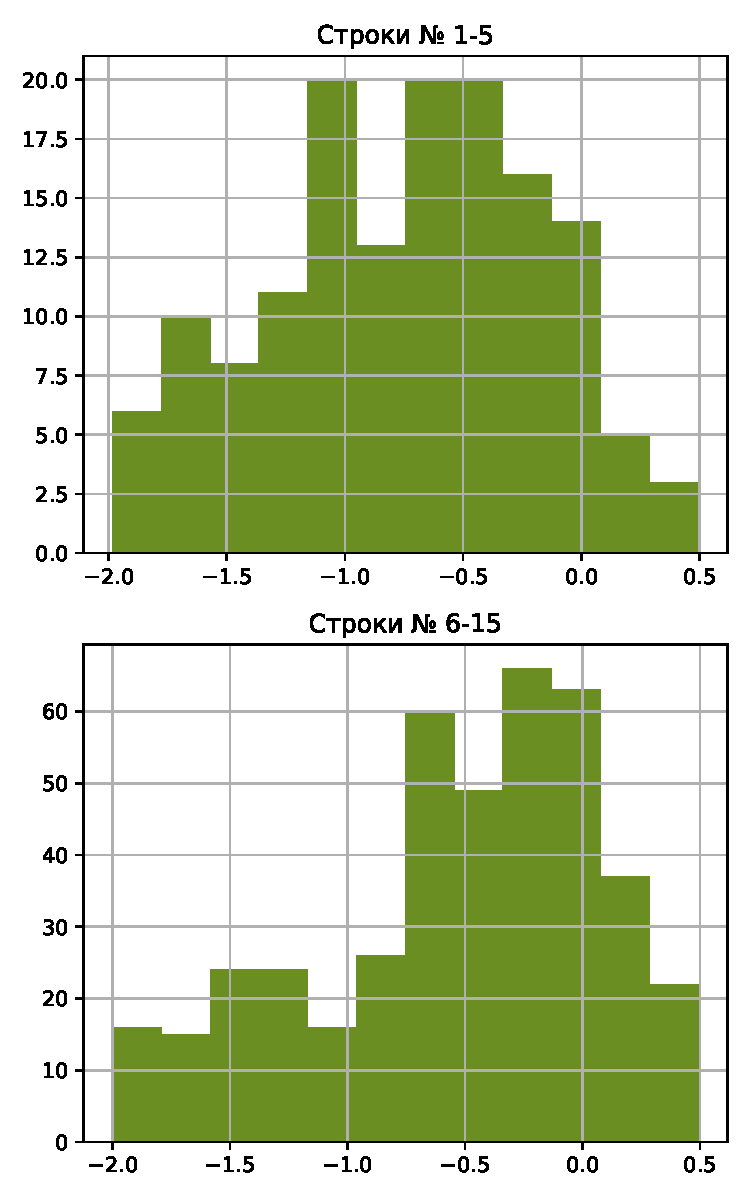
\includegraphics[scale=0.5]{distr_curv.pdf}
\end{minipage}
\caption{Рукописный текст и его распределение величины наклона по строкам.}
\end{figure}

\subsubsection{Признак-кривизна}
Вторую фундаментальную характеристику письма, кривизну, можно определить следующим образом. Будем считать элементарную степень кривизны трёх последовательно взятых точек, как разность суммы расстояний между соседними точками и расстояния между крайними. Итоговую величину положим равной сумме всех таких элементарных степеней кривизны. Формульно это записывается так:

\begin{equation}
\emph{curvature} = \sum_{i=2}^{N-1}(dist(p_{i-1}, p_{i}) + dist(p_{i}, p_{i+1}) - dist(p_{i-1}, p_{i+1})),
\end{equation}

\begin{equation}
dist(p(x_1, y_1), p(x_2, y_2)) = \sqrt{(x_1 - x_2)^2 + (y_1 - y_2)^2}
\end{equation}

Установим зависимость построенного признака-кривизны на том же изображении с двумя почерками (рис.5). Первый почерк можно охарактеризовать как прерывистый. Штрихи в нём в большей степени представляют линии, нарисованные между последовательными отрываниями руки от листа. При таком стиле писания особенно наглядно возникает определённый набор шаблонов писателя. Из элементов такого набора и состоит каждый рисуемый символ. Так, на графике рис.5 видно, что штрихи по величине кривизны разбиваются на три отделимых кластера по значению: 0-2, 2-5, 6-10. Второй почерк таким свойством не обладает, написанный им текст имеет межсимвольные переходы, более гладкую форму, в следствие чего и распределение получается более гладким.

\begin{figure}[h]
\begin{minipage}[h]{0.5\linewidth}
    \centering
    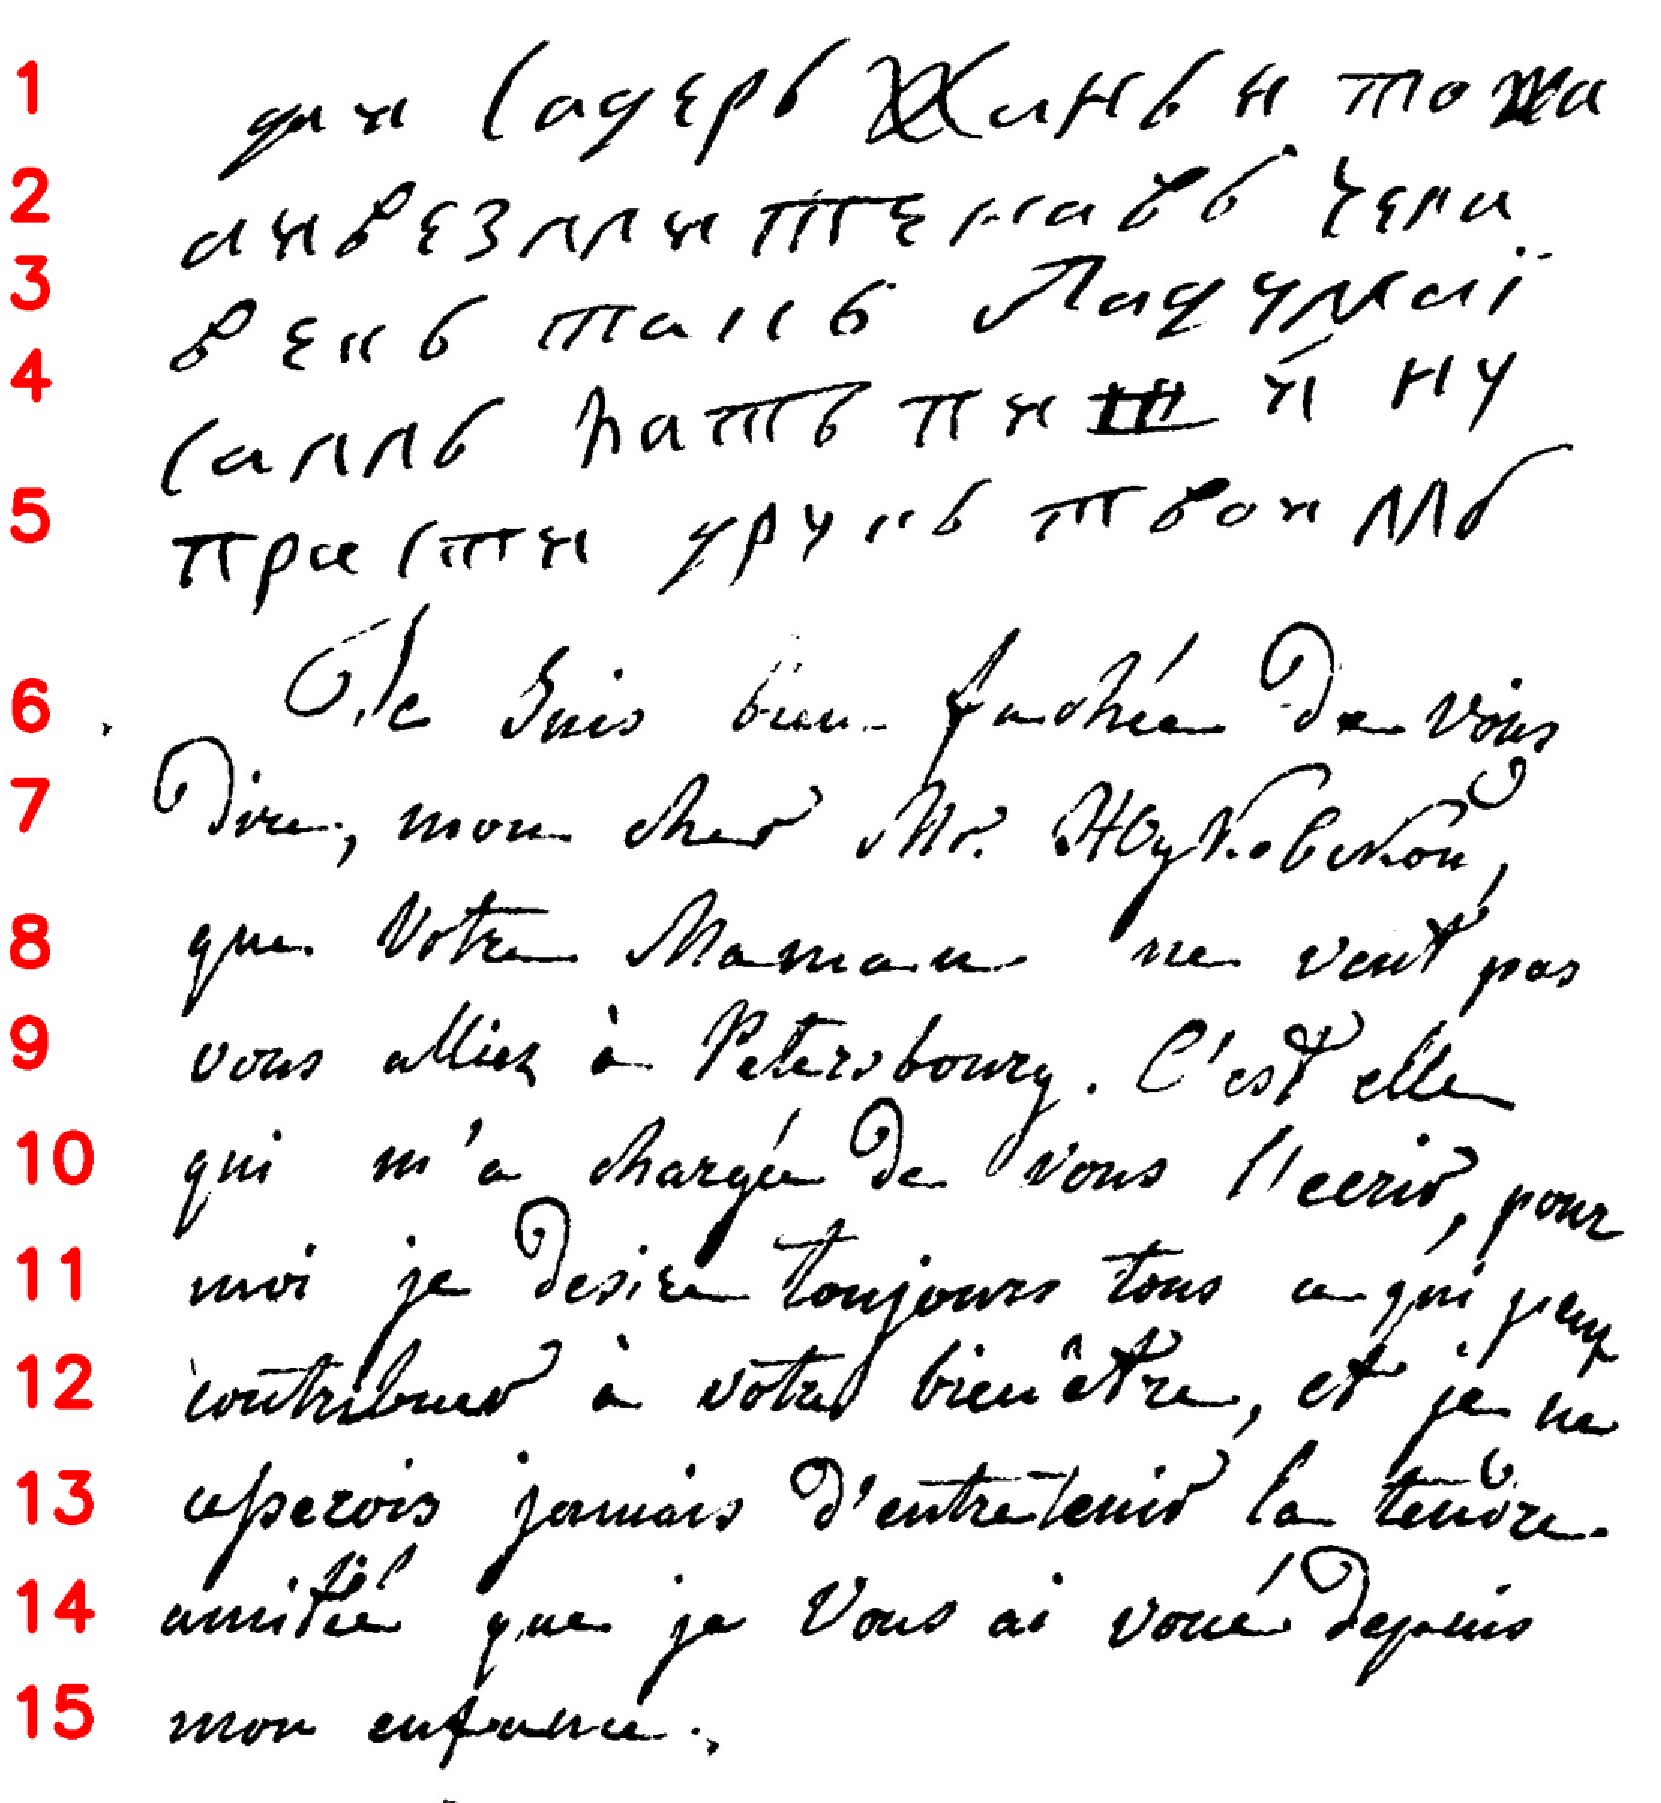
\includegraphics[scale=0.26]{afterotsu-cropped.pdf} 
\end{minipage}
\hfill
\begin{minipage}[h]{0.46\linewidth}
    \centering
    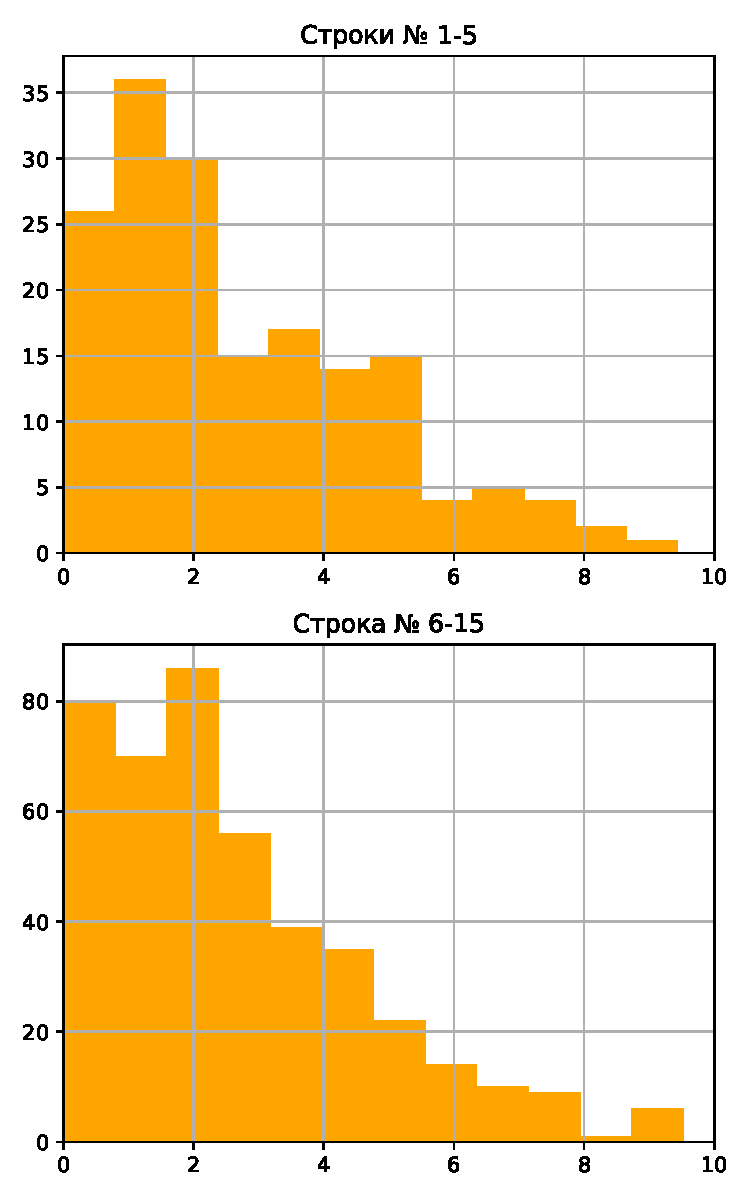
\includegraphics[scale=0.5]{distr_inc.pdf}
\end{minipage}
\caption{Рукописный текст и его распределение величины кривизны по строкам.}
\end{figure}

Рассмотренные классические признаки оказались чувствительны к разным почеркам, поэтому можно утверждать о состоятельности данного штрихового представления.

\subsection{Особенность почерка: кольцевые штрихи}
Предлагается обратить внимание на возможность классификации штрихов по типу: цепь, кольцо или отрезок. Наиболее способным отразить стиль почерка писателя можно назвать кольцевой тип штриха, ведь помимо того, что данный тип можно охарактерирозвать метрическими признаками: наклоном, кривизной или размером - каждому почерку свойственна своя частота встречаемости такого типа. Имеется в виду, что одни и те же буквы можно писать с петлёй и без (рис.1), и такие петли относятся к кольцевым штрихам. 

В данной части работы построим признаки, характеризующие кольцевой тип штрихов. 

На рис.6 представлены выделенные кольцевые штрихи исследуемого представления. Можно заметить, что детектируются не все распознаваемые глазом кольцевые штрихи, но тем не менее значительная их часть, по которой возможно провести анализ, приводящий к результату.

\begin{figure}[h]
\begin{minipage}[h]{0.47\linewidth}
    \centering
    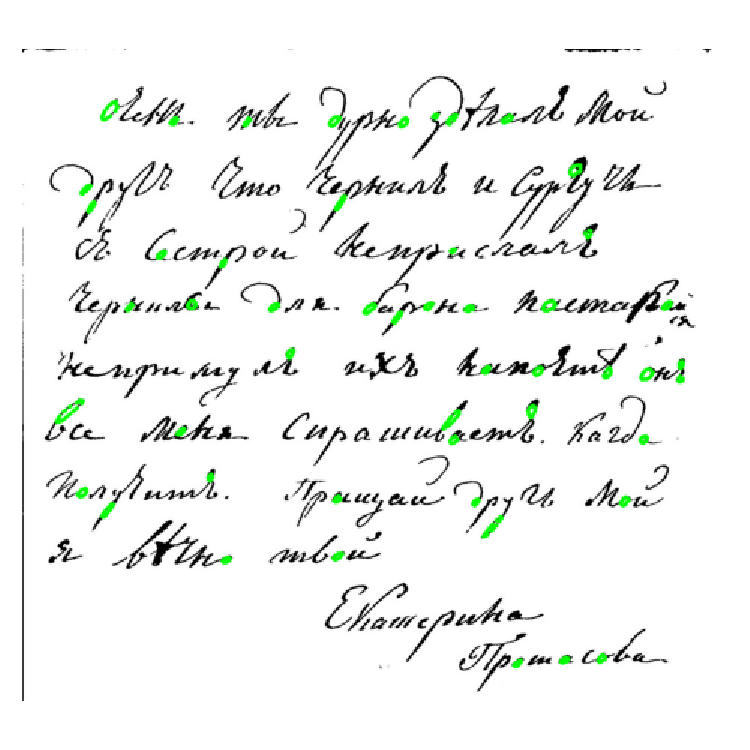
\includegraphics[scale=0.7]{ringsall.pdf} \\Все
\end{minipage}
\hfill
\begin{minipage}[h]{0.47\linewidth} 
    \centering
    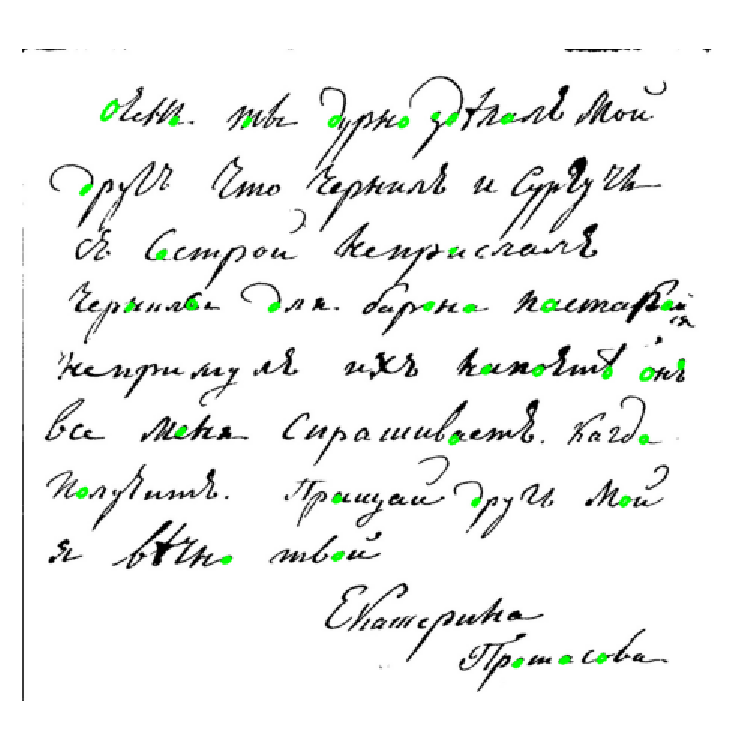
\includegraphics[scale=0.7]{ringsbase.pdf} \\Базовые
\end{minipage}
\caption{Пример кольцевых штрихов.}
\end{figure}

На рис.7 приведены примеры разных почерков. Обращая внимание на кольцевые штрихи, можно заметить, что у первого почерка рассматриваемые элементы ближе к форме кольца, отчётливо видна "дырка". У второго же почерка такие штрихи меньше и больше напоминают форму овала. Предлагается построить признаки, отражающие данные различия. 

\begin{figure}[h]
\begin{minipage}[h]{1\linewidth}
\center{\includegraphics[width=0.8\linewidth]{Почерк 2_2.jpg}}
\end{minipage}
\vfill
\begin{minipage}[h]{1\linewidth}
\center{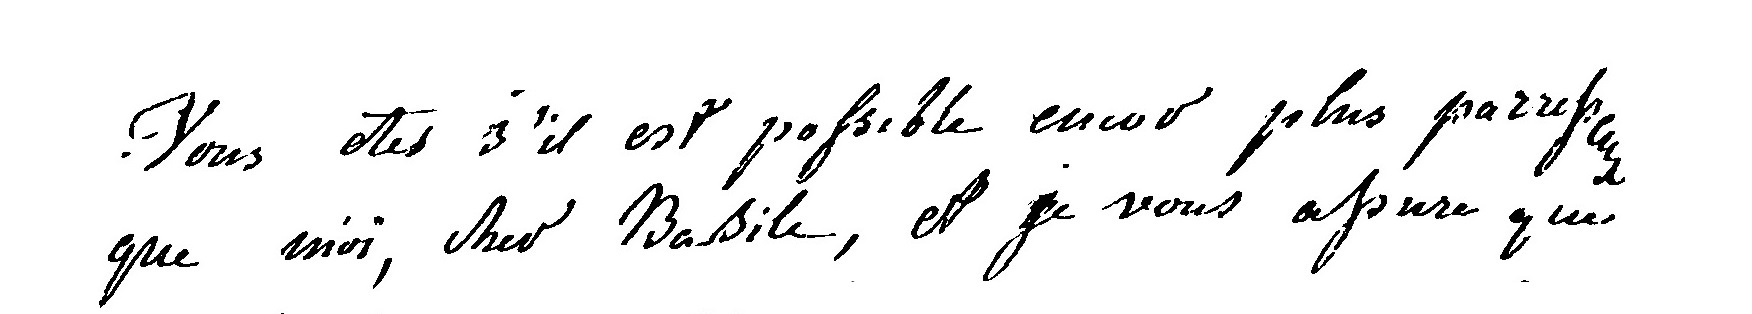
\includegraphics[width=0.8\linewidth]{Почерк 4_1.jpg}}
\end{minipage}
\caption{Пример разных почерков.}
\end{figure}

\subsubsection{Признак-форма}
Рассматриваемые в этом разделе штрихи имеют эллиптическую структуру, поэтому 
признак-форму можно определить как отношение большой полуоси к малой. Чем данная величина ближе к единице, тем штрих больше напоминает кольцо.

Длины полуосей эллипса определим следующим образом (5)-(7). Найдём приближённый центр, а затем из набора точек, входящих в штрих, найдём такие точки, расстояния до которых было бы наибольшим и наименьшим. Эти расстояние и будут определять большую и малую полуоси соответсвтенно. Как и раньше, будем считать евклидово расстояние между двумя точками (4).

\begin{equation}
    x_c = \mathbb{E}x,~y_c = \mathbb{E}y,~p_c(x_c, y_c) = (x_c, y_c)
\end{equation}

\begin{equation}
    a =\max\limits_{i \in {1,...,N}} dist(p_i, p_c)
\end{equation}

\begin{equation}
    b =\min\limits_{i \in {1,...,N}} dist(p_i, p_c)
\end{equation}

Тогда итоговая величина, отражающая форму штриха, будет определяться формулой (8).

\begin{equation}
    \emph{shape} = \frac{a}{b}
\end{equation}

\subsubsection{Признак-размер}
Аналогично форме штриха определим величину его размера (9). Домножение на $\pi$ осуществляется для интерпретируемости настоящей площади эллипса.

\begin{equation}
    \emph{area} = a b \pi
\end{equation}

\subsubsection{Признак-частота}
Как видно будет далее, построенное к настоящему моменту признаковое пространство позволяет идентифицировать различные почерки, но некоторые стили писания сливаются. Поэтому остаётся необходимость в большем количестве признаков. 

Так же как писатель может сделать петлю в том месте, где не сделает её другой автор, он может делать отличительно выступающие за базовую линию штрихи в разных местах. Поэтому предлагается добавить признак, отвечающий за частоту встречаемости выступающих штрихов по отношению к другим для каждой строки (10), где $M$ - число строк, $K_i$ - количество штрихов в $i$-ой строке.

\begin{equation}
    \emph{ledge} = \frac{1}{M} \sum_{i=1}^{M} \frac{\sum_{j=1}^{K_i}[stroke_j = '\text{выступающий}']}{K_i}
\end{equation}

\section{Вычислительный эксперимент}
Оценим возможность классифицировать почерк по отдельным штрихам на основе построенных признаков. Эксперимент будет заключаться в классификации четырёх почерков: 5 изображений первого почерка, 3 - второго, 5 - третьего, 3 - четвёртого, - преимущественно опираясь на особенности кольцевых штрихов. Примеры двух типов почерков представлены на рис.7, со всеми рассматриваемыми типами можно ознакомиться в приложении.

Будем оценивать наиболее часто встречающиеся кольцевые штрихи: оставим для рассмотрения только базовые штрихи с не слишком вытянутой формой (shape < 10) и выбросим 15\% самых больших. Полученные значения признаков для рассматриваемых почерков приведены в Таблице 1.

\begin{table}[!h]
    \centering
    \begin{tabular}{|p{4cm}||p{3cm}|p{3cm}|p{3cm}|}
        \hline
        Тип почерка & \emph{shape} & \emph{area} & \emph{ledge}\\ 
        \hline\hline
        1 & 5.73 & 81 & 0.108 \\
        1 & 7.30 & 75 & 0.085 \\
        1 & 6.15 & 83 & 0.050 \\
        1 & 4.11 & 105 & 0.133 \\
        1 & 5.64 & 77 & 0.107 \\
        \hline
        2 & - & 220 & - \\
        2 & - & 178 & - \\
        2 & - & 188 & - \\
        \hline
        3 & 4.42 & 93 & 0.141 \\
        3 & 3.83 & 82 & 0.121 \\
        3 & 4.41 & 86 & 0.124 \\
        3 & 4.58 & 140 & 0.13 \\
        3 & 5.20 & 81 & 0.135 \\
        \hline
        4 & 6.82 & 132 & 0.041 \\
        4 & 6.32 & 102 & 0.022 \\
        4 & 6.33 & 107 & 0.154 \\
        \hline
    \end{tabular}
    \caption{Значения признаков для разных почерков.}
\end{table}

Анализируя полученные результаты, однозначно можно опредлить второй тип почерка по размеру кольцевых штрихов, эти значения самые большие среди рассматриваемых типов почерков. Также можно заметить, что по форме этих штрихов можно отличить, за исключением одного объекта, 3-ий тип почерка от 4-ого, по размеру - 1-ый от 4-ого и по частоте выступающих штрихов - 1-ый от 3-его. Что в итоге позволяет определить тип каждого отдельного почерка. 

Рассмотрим поближе четвёртый объект из таблицы (1 тип почерка), который классифицируется неправильно (рис. 8). У данного фрагмента почерка кольцевых штрихов немного, в частности, слишком маленькая выборка базовых штрихов. Вследствие чего значениями признаков данный фрагмент классифицируется как почерк 3-его типа.

Из эксперимента можно сделать вывод, что построенные признаки являются чувствительными к оценке возможности классифицировать почерк на выделенных штрихах. В частности, специфика кольцевых штрихов была установлена как особенность каждого писателя, позволяющая различать разных авторов. Однако такой подход является переобученным и далеко не все признаки показывают значения, по которым можно примерно отличать каждый почерк от других. Требуется строить более сложные конструкции, учитывающие разные аспекты письма. Кроме того, обучение должно происходить на большом объёме изображений почерков, когда величины каждого признака почерка будут объективно отражать исследуемые характеристики. Вместе с тем входные изображения должны представлять собой хотя бы несколько строк текста, иначе алгоритм будет работать некорректно.

\begin{figure}[h]
\begin{minipage}[h]{1\linewidth}
\center{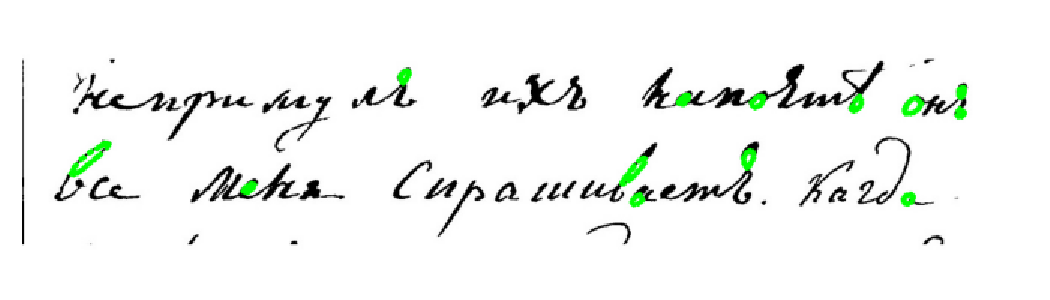
\includegraphics[width=0.7\linewidth]{err.pdf}} \\ Кольцевые штрихи
\end{minipage}
\vfill
\begin{minipage}[h]{1\linewidth}
\center{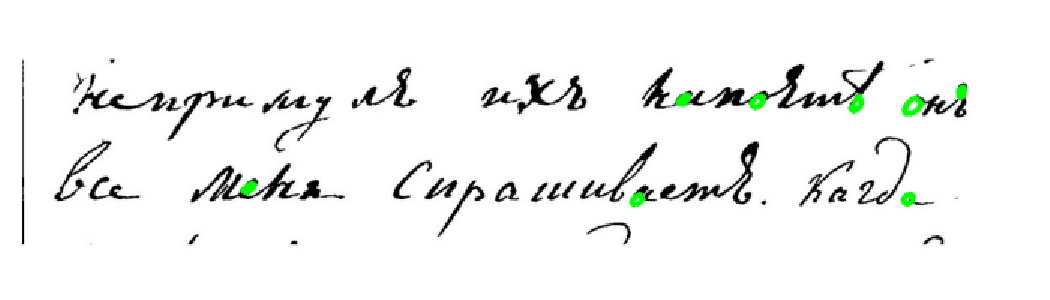
\includegraphics[width=0.7\linewidth]{errbase.pdf}} \\ Базовые штрихи
\end{minipage}
\caption{Изображение, на котором происходит ошибка.}
\end{figure}

\section{Заключение}
В данной работе были построены метрические признаки строк и признаки, основанные на штриховом представлении рукописного текста, с помощью которых была установлена возможность классифицировать почерки разных писателей. Был проведён вычислительный эксперимент, в ходе которого осуществлённый подход решил поставленную задачу и были выявлены недостатки. Совокупость этих недостатков и того факта, что были рассмотрены не все аспекты штрихового представления, а только его часть, дают задел на будущие исследования.

\newpage

% \section{Headings: first level}
% \label{sec:headings}

% \lipsum[4] See Section \ref{sec:headings}.

% \subsection{Headings: second level}
% \lipsum[5]
% \begin{equation}
% 	\xi _{ij}(t)=P(x_{t}=i,x_{t+1}=j|y,v,w;\theta)= {\frac {\alpha _{i}(t)a^{w_t}_{ij}\beta _{j}(t+1)b^{v_{t+1}}_{j}(y_{t+1})}{\sum _{i=1}^{N} \sum _{j=1}^{N} \alpha _{i}(t)a^{w_t}_{ij}\beta _{j}(t+1)b^{v_{t+1}}_{j}(y_{t+1})}}
% \end{equation}

% \subsubsection{Headings: third level}
% \lipsum[6]

% \paragraph{Paragraph}
% \lipsum[7]



% \section{Examples of citations, figures, tables, references}
% \label{sec:others}

% \subsection{Citations}
% Citations use \verb+natbib+. The documentation may be found at
% \begin{center}
% 	\url{http://mirrors.ctan.org/macros/latex/contrib/natbib/natnotes.pdf}
% \end{center}

% Here is an example usage of the two main commands (\verb+citet+ and \verb+citep+): Some people thought a thing \citep{kour2014real, hadash2018estimate} but other people thought something else \citep{kour2014fast}. Many people have speculated that if we knew exactly why \citet{kour2014fast} thought this\dots

% \subsection{Figures}
% \lipsum[10]
% See Figure \ref{fig:fig1}. Here is how you add footnotes. \footnote{Sample of the first footnote.}
% \lipsum[11]

% \begin{figure}
% 	\centering
% 	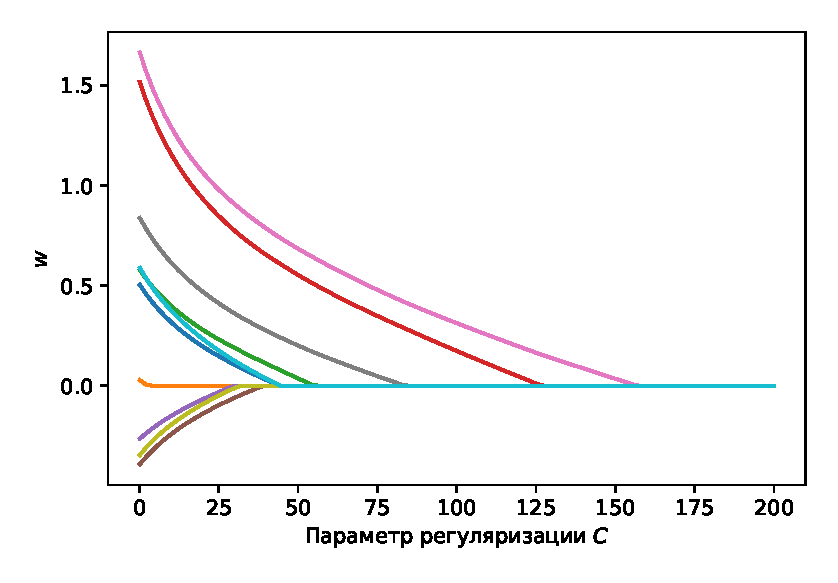
\includegraphics[width=0.5\textwidth]{../figures/log_reg_cs_exp.eps}
% 	\caption{Sample figure caption.}
% 	\label{fig:fig1}
% \end{figure}

% \subsection{Tables}
% See awesome Table~\ref{tab:table}.

% The documentation for \verb+booktabs+ (`Publication quality tables in LaTeX') is available from:
% \begin{center}
% 	\url{https://www.ctan.org/pkg/booktabs}
% \end{center}


% \begin{table}
% 	\caption{Sample table title}
% 	\centering
% 	\begin{tabular}{lll}
% 		\toprule
% 		\multicolumn{2}{c}{Part}                   \\
% 		\cmidrule(r){1-2}
% 		Name     & Description     & Size ($\mu$m) \\
% 		\midrule
% 		Dendrite & Input terminal  & $\sim$100     \\
% 		Axon     & Output terminal & $\sim$10      \\
% 		Soma     & Cell body       & up to $10^6$  \\
% 		\bottomrule
% 	\end{tabular}
% 	\label{tab:table}
% \end{table}

% \subsection{Lists}
% \begin{itemize}
% 	\item Lorem ipsum dolor sit amet
% 	\item consectetur adipiscing elit.
% 	\item Aliquam dignissim blandit est, in dictum tortor gravida eget. In ac rutrum magna.
% \end{itemize}

\nocite{*}
\bibliographystyle{plain}
\bibliography{references}

\end{document}
